\chapter{Kết quả thực nghiệm}

\section{Môi trường thử nghiệm}

\begin{itemize}
    \item \textbf{Hệ điều hành:} Ubuntu 24.04 (Noble Numbat)
    \item \textbf{Trình biên dịch:} g++ (GCC) 13.2.0
    \item \textbf{Tiêu chuẩn C++:} C++17
    \item \textbf{CPU:} x86\_64
\end{itemize}

\section{Kết quả các test case}

Chương trình được kiểm tra với 7 bộ dữ liệu đầu vào. Dưới đây là kết quả biểu đồ Gantt cho từng bộ.

\subsection{Test case 1: \texttt{input\_basic.txt} (FCFS)}

Đầu vào: 3 tiến trình với chu kỳ CPU-R đan xen.

\begin{itemize}
    \item P1: đến 0, bursts [CPU 5, R 3, CPU 2, R 2]
    \item P2: đến 2, bursts [CPU 4, R 2]
    \item P3: đến 5, bursts [CPU 3, R 1, CPU 2, R 1]
\end{itemize}

\begin{verbatim}
CPU: 1 1 1 1 1 2 2 2 2 3 3 3 1 1 3 3 _ _
R  : _ _ _ _ _ _ 1 1 1 _ 2 2 _ 3 _ 1 1 3
\end{verbatim}

Tổng thời gian mô phỏng: 18 ticks. CPU utilization: 88,88\%. Resource utilization: 50,00\%.

\begin{table}[h]
\centering
\begin{tabular}{|c|c|c|c|}
\hline
PID & Response (s) & Waiting (s) & Turnaround (s) \\
\hline
P1 & 0,00 & 4,00 & 17,00 \\
P2 & 3,00 & 3,00 & 10,00 \\
P3 & 4,00 & 5,00 & 13,00 \\
\hline
TB & 2,33 & 4,00 & 13,33 \\
\hline
\end{tabular}
\caption{Kết quả test case 1}
\end{table}

\subsection{Test case 2: \texttt{input\_simple.txt} (FCFS)}

Đầu vào: 2 tiến trình CPU-only.

\begin{itemize}
    \item P1: đến 0, bursts [CPU 3]
    \item P2: đến 1, bursts [CPU 5]
\end{itemize}

\begin{verbatim}
CPU: 1 1 1 2 2 2 2 2
R  : _ _ _ _ _ _ _ _
\end{verbatim}

CPU utilization: 100\%. Resource utilization: 0\%.

\begin{table}[h]
\centering
\begin{tabular}{|c|c|c|c|}
\hline
PID & Response (s) & Waiting (s) & Turnaround (s) \\
\hline
P1 & 0,00 & 0,00 & 3,00 \\
P2 & 2,00 & 2,00 & 7,00 \\
\hline
TB & 1,00 & 1,00 & 5,00 \\
\hline
\end{tabular}
\caption{Kết quả test case 2}
\end{table}

\subsection{Test case 3: \texttt{input\_fcfs.txt} (FCFS)}

Đầu vào: 3 tiến trình với resource R.

\begin{itemize}
    \item P1: đến 0, bursts [CPU 5, R 2]
    \item P2: đến 2, bursts [CPU 3]
    \item P3: đến 4, bursts [CPU 4, R 3]
\end{itemize}

\begin{verbatim}
CPU: 1 1 1 1 1 2 2 2 3 3 3 3 _ _ _ _
R  : _ _ _ _ _ _ 1 1 _ _ _ _ _ 3 3 3
\end{verbatim}

CPU utilization: 75\%. Resource utilization: 31,25\%.

\begin{table}[h]
\centering
\begin{tabular}{|c|c|c|c|}
\hline
PID & Response (s) & Waiting (s) & Turnaround (s) \\
\hline
P1 & 0,00 & 0,00 & 8,00 \\
P2 & 3,00 & 3,00 & 6,00 \\
P3 & 4,00 & 4,00 & 12,00 \\
\hline
TB & 2,33 & 2,33 & 8,67 \\
\hline
\end{tabular}
\caption{Kết quả test case 3}
\end{table}

\subsection{Test case 4: \texttt{input\_rr.txt} (RR, quantum = 2)}

Đầu vào: 3 tiến trình CPU-only đến cùng lúc.

\begin{itemize}
    \item P1: đến 0, bursts [CPU 6]
    \item P2: đến 0, bursts [CPU 3]
    \item P3: đến 0, bursts [CPU 4]
\end{itemize}

\begin{verbatim}
CPU: 1 1 2 2 3 3 1 1 2 3 3 1 1
R  : _ _ _ _ _ _ _ _ _ _ _ _ _
\end{verbatim}

CPU utilization: 100\%. Resource utilization: 0\%.

\begin{table}[h]
\centering
\begin{tabular}{|c|c|c|c|}
\hline
PID & Response (s) & Waiting (s) & Turnaround (s) \\
\hline
P1 & 0,00 & 9,00 & 13,00 \\
P2 & 2,00 & 7,00 & 9,00 \\
P3 & 4,00 & 8,00 & 11,00 \\
\hline
TB & 2,00 & 8,00 & 11,00 \\
\hline
\end{tabular}
\caption{Kết quả test case 4}
\end{table}

\subsection{Test case 5: \texttt{input\_sjf.txt} (SJF)}

Đầu vào: 4 tiến trình CPU-only đến so le.

\begin{itemize}
    \item P1: đến 0, bursts [CPU 8]
    \item P2: đến 1, bursts [CPU 4]
    \item P3: đến 2, bursts [CPU 2]
    \item P4: đến 3, bursts [CPU 1]
\end{itemize}

\begin{verbatim}
CPU: 1 1 1 1 1 1 1 1 4 3 3 2 2 2 2
R  : _ _ _ _ _ _ _ _ _ _ _ _ _ _ _
\end{verbatim}

CPU utilization: 100\%. Resource utilization: 0\%.

\begin{table}[h]
\centering
\begin{tabular}{|c|c|c|c|}
\hline
PID & Response (s) & Waiting (s) & Turnaround (s) \\
\hline
P1 & 0,00 & 0,00 & 8,00 \\
P2 & 10,00 & 10,00 & 14,00 \\
P3 & 7,00 & 7,00 & 9,00 \\
P4 & 5,00 & 5,00 & 6,00 \\
\hline
TB & 5,50 & 5,50 & 9,25 \\
\hline
\end{tabular}
\caption{Kết quả test case 5}
\end{table}

\subsection{Test case 6: \texttt{input\_srtn.txt} (SRTN)}

Đầu vào: 3 tiến trình CPU-only đến so le.

\begin{itemize}
    \item P1: đến 0, bursts [CPU 8]
    \item P2: đến 1, bursts [CPU 3]
    \item P3: đến 2, bursts [CPU 2]
\end{itemize}

\begin{verbatim}
CPU: 1 2 2 2 3 3 1 1 1 1 1 1 1
R  : _ _ _ _ _ _ _ _ _ _ _ _ _
\end{verbatim}

CPU utilization: 100\%. Resource utilization: 0\%.

\begin{table}[h]
\centering
\begin{tabular}{|c|c|c|c|}
\hline
PID & Response (s) & Waiting (s) & Turnaround (s) \\
\hline
P1 & 0,00 & 5,00 & 13,00 \\
P2 & 0,00 & 0,00 & 3,00 \\
P3 & 2,00 & 2,00 & 4,00 \\
\hline
TB & 0,67 & 2,33 & 6,67 \\
\hline
\end{tabular}
\caption{Kết quả test case 6}
\end{table}

\subsection{Test case 7: \texttt{input\_bug2\_srtn.txt} (SRTN)}

Đầu vào: 2 tiến trình, P1 có chu kỳ CPU-R-CPU.

\begin{itemize}
    \item P1: đến 0, bursts [CPU 2, R 1, CPU 8]
    \item P2: đến 1, bursts [CPU 5]
\end{itemize}

\begin{verbatim}
CPU: 1 2 2 2 2 2 1 _ 1 1 1 1 1 1 1 1
R  : _ _ _ _ _ _ _ _ 1 _ _ _ _ _ _ _
\end{verbatim}

CPU utilization: 93,75\%. Resource utilization: 6,25\%.

\begin{table}[h]
\centering
\begin{tabular}{|c|c|c|c|}
\hline
PID & Response (s) & Waiting (s) & Turnaround (s) \\
\hline
P1 & 0,00 & 5,00 & 16,00 \\
P2 & 0,00 & 0,00 & 5,00 \\
\hline
TB & 0,00 & 2,50 & 10,50 \\
\hline
\end{tabular}
\caption{Kết quả test case 7}
\end{table}

\section{So sánh các thuật toán}

Để so sánh các thuật toán, chúng tôi sử dụng test case 4 (input\_rr.txt) -- 3 tiến trình đến cùng lúc -- và test case 6 (input\_srtn.txt) -- 3 tiến trình đến so le -- vì đây là các kịch bản thể hiện rõ sự khác biệt giữa các thuật toán.

\subsection{So sánh trên test case 4 (cùng đến)}

\begin{table}[h]
\centering
\begin{tabular}{|c|c|c|c|c|}
\hline
Thuật toán & RT TB & WT TB & TAT TB & CPU Util \\
\hline
FCFS & 0,00 & 5,00 & 9,67 & 100\% \\
RR (q=2) & 2,00 & 8,00 & 11,00 & 100\% \\
SJF & 0,00 & 5,00 & 9,67 & 100\% \\
SRTN & 0,00 & 5,00 & 9,67 & 100\% \\
\hline
\end{tabular}
\caption{So sánh các thuật toán trên test case 4}
\end{table}

Khi tất cả tiến trình đến cùng lúc, SJF và SRTN cho kết quả tương đương FCFS (đều chạy P1 trước). RR có waiting time và turnaround time cao hơn do overhead của preemption và context-switch.

\subsection{So sánh trên test case 6 (đến so le)}

\begin{table}[h]
\centering
\begin{tabular}{|c|c|c|c|c|}
\hline
Thuật toán & RT TB & WT TB & TAT TB & CPU Util \\
\hline
FCFS & 1,33 & 4,67 & 9,00 & 100\% \\
RR (q=2) & 1,33 & 5,00 & 9,33 & 100\% \\
SJF & 0,67 & 2,33 & 6,67 & 100\% \\
SRTN & 0,67 & 2,33 & 6,67 & 100\% \\
\hline
\end{tabular}
\caption{So sánh các thuật toán trên test case 6}
\end{table}

Khi tiến trình đến so le với burst length khác nhau, SJF và SRTN cho thấy ưu thế vượt trội: waiting time giảm gần một nửa so với FCFS và RR.

\begin{figure}[h]
\centering
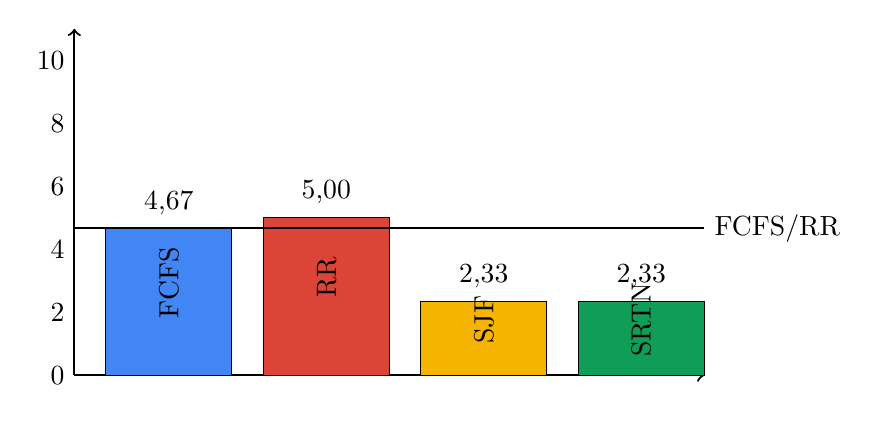
\begin{tikzpicture}[scale=0.8]
\definecolor{bar1}{RGB}{66,133,244}
\definecolor{bar2}{RGB}{219,68,55}
\definecolor{bar3}{RGB}{244,180,0}
\definecolor{bar4}{RGB}{15,157,88}

% Axes
\draw[thick,->] (0,0) -- (10,0);
\draw[thick,->] (0,0) -- (0,5.5);

% Labels
\node[left] at (0,0) {0};
\node[left] at (0,1) {2};
\node[left] at (0,2) {4};
\node[left] at (0,3) {6};
\node[left] at (0,4) {8};
\node[left] at (0,5) {10};

% FCFS
\draw[fill=bar1] (0.5,0) rectangle (2.5,{4.67/2});
\node[rotate=90] at (1.5,{4.67/4+0.3}) {FCFS};
\node at (1.5,{4.67/2+0.4}) {4,67};

% RR
\draw[fill=bar2] (3,0) rectangle (5,{5.0/2});
\node[rotate=90] at (4,{5.0/4+0.3}) {RR};
\node at (4,{5.0/2+0.4}) {5,00};

% SJF
\draw[fill=bar3] (5.5,0) rectangle (7.5,{2.33/2});
\node[rotate=90] at (6.5,{2.33/4+0.3}) {SJF};
\node at (6.5,{2.33/2+0.4}) {2,33};

% SRTN
\draw[fill=bar4] (8,0) rectangle (10,{2.33/2});
\node[rotate=90] at (9,{2.33/4+0.3}) {SRTN};
\node at (9,{2.33/2+0.4}) {2,33};

\draw[thick] (0,{4.67/2}) -- (10,{4.67/2}) node[right] {FCFS/RR};

\end{tikzpicture}
\caption{So sánh Waiting Time trung bình giữa các thuật toán (test case 6)}
\label{fig:wt-comparison}
\end{figure}

\subsection{Nhận xét}

\begin{enumerate}
    \item \textbf{SJF và SRTN} cho kết quả vượt trội về waiting time và turnaround time so với FCFS và RR, đặc biệt khi các tiến trình có burst length chênh lệch lớn.
    \item \textbf{Round Robin} có waiting time cao nhất do cơ chế preemption định kỳ, nhưng đảm bảo tính công bằng -- không tiến trình nào bị starvation.
    \item \textbf{FCFS} đơn giản nhưng dễ bị hiệu ứng convoy: tiến trình CPU burst dài ở đầu hàng đợi sẽ làm tăng waiting time của các tiến trình khác.
    \item \textbf{CPU Utilization} đạt 100\% trong hầu hết test case CPU-only. Với các test case có resource R, utilization thấp hơn do CPU phải chờ resource.
\end{enumerate}
